\documentclass[t]{beamer}
\usepackage[utf8]{inputenc}  % to be able to type unicode text directly
%\usepackage[french]{babel}   % french typographical conventions
\usepackage{inconsolata}     % for a nicer (e.g. non-courier) tt family font
%\usepackage{amsthm,amsmath}  % fancier mathematics
\usepackage{array} % to fine-tune tabular spacing
\usepackage{bbm} % for blackboard 1

\usepackage{graphicx}        % to include images
%\usepackage{animate}         % to include animated images
\usepackage{soul}            % for colored strikethrough
%\usepackage{bbding}          % for Checkmark and XSolidBrush
\usepackage{hyperref,url}

\colorlet{darkgreen}{black!50!green}  % used for page numbers
\definecolor{term}{rgb}{.9,.9,.9}     % used for code insets

\setlength{\parindent}{0em}
\setlength{\parskip}{1em}


% coco's macros
\newcommand{\ds}{\displaystyle}
\def\R{\textbf{R}}
\def\C{\textbf{C}}
\def\K{\textbf{K}}
\def\N{\textbf{N}}
\def\F{\mathcal{F}}
\def\x{\textbf{x}}
\def\y{\mathbf{y}}
\def\u{\mathbf{u}}
\def\Z{\textbf{Z}}
\def\d{\mathrm{d}}
\DeclareMathOperator*{\argmin}{arg\,min}
\DeclareMathOperator*{\argmax}{arg\,max}
\newcommand{\reference}[1] {{\scriptsize \color{gray}  #1 }}
\newcommand{\referencep}[1] {{\tiny \color{gray}  #1 }}
\newcommand{\unit}[1] {{\tiny \color{gray}  #1 }}

% matrix groups and sets
\newcommand{\M}{\mathrm{M}}
\newcommand{\GL}{\mathrm{GL}}
\newcommand{\TS}{\mathrm{TS}}
\newcommand{\TI}{\mathrm{TI}}
\newcommand{\UU}{\mathrm{U}}
\newcommand{\OO}{\mathrm{O}}
\newcommand{\SO}{\mathrm{SO}}
\newcommand{\SU}{\mathrm{SU}}
\newcommand{\SL}{\mathrm{SL}}
\newcommand{\SSS}{\mathrm{S}}
\newcommand{\HH}{\mathrm{H}}

\newcommand{\parens}[1]{\left(#1\right)} % (x)
\newcommand{\pairing}[2]{\left\langle #1,#2\right\rangle} % <x,y>

% \abs{x}   ->    |x|
% \Abs{x}   ->   ||x||
% \ABS{x}   ->  |||x|||
\newcommand{\abs}[1]{\left|#1\right|}
\newcommand{\Abs}[1]{\left\|#1\right\|}
\newcommand{\ABS}[1]{{\left\vert\kern-0.25ex\left\vert\kern-0.25ex\left\vert #1 \right\vert\kern-0.25ex\right\vert\kern-0.25ex\right\vert}}

% disable spacing around verbatim
\usepackage{etoolbox}
\makeatletter\preto{\@verbatim}{\topsep=0pt \partopsep=0pt }\makeatother

% disable headings, set slide numbers in green
\mode<all>\setbeamertemplate{navigation symbols}{}
\defbeamertemplate*{footline}{pagecount}{\leavevmode\hfill\color{darkgreen}
   \insertframenumber{} / \inserttotalframenumber\hspace*{2ex}\vskip0pt}

%% select red color for strikethrough
\makeatletter
\newcommand\SoulColor{%
  \let\set@color\beamerorig@set@color
  \let\reset@color\beamerorig@reset@color}
\makeatother
\newcommand<>{\St}[1]{\only#2{\SoulColor\st{#1}}}
\setstcolor{red}

% make everything monospace
\renewcommand*\familydefault{\ttdefault}

\begin{document}

\begin{frame}[plain,fragile]
\LARGE
\begin{verbatim}




        ANALYSE NUMÉRIQUE 4/6
        Algèbre linéaire numérique




EML
16--11--2020
\end{verbatim}
\end{frame}

\begin{frame}[fragile]
PLAN\\
====

1. Aperçu des résultats principaux ({\bf 20min})

2. Travail par groupes ({\bf 90min})

3. Mise en commun ({\bf 60min})

\vfill
S.V.P.~: veuillez envoyer des retours (même anonymes) sur cette organisation à
\color{blue}\verb+enric.meinhardt@ens-paris-saclay.fr+
\vfill
\end{frame}

\begin{frame}
INTRO: LES 4 PROBLÈMES DE L'ALGÈBRE LINÉAIRE NUMÉRIQUE\\
======================================================

%Il y a seulement 4 problèmes en algèbre linéaire numérique.
Étant~$A\in\mathcal{M}_{m,n}(\K)$ de rang complet, %il faut
trouver~${\color{red}\x}\in\K^n$~:

{\color{blue} 1.}
\fbox{$A{\color{red}\x}=b,\quad A\in\mathcal{M}_{n,n}(\K)$}
\pause
Solution:~$x=A^{-1}b$.

\pause
{\color{blue} 2.}
\fbox{$A{\color{red}\x}=b,\quad A\in\mathcal{M}_{m,n}(\K),\ m<n$}
\pause
Système sous-déterminé, espace affine de solutions.  Si~$A=[Q|S]$ alors
$x=\left[Q^{-1}b-Q^{-1}S\mu\ |\ \mu\right]$ est solution~$\forall \mu\in\R^{n-m}$.

\pause
{\color{blue} 3.}
\fbox{$A{\color{red}\x}=b,\quad A\in\mathcal{M}_{m,n}(\K),\ m>n$}
\pause
Système surdéterminé, pas de solution en général.
\pause
``Solution'' de moindres
carrées: $\arg\min_x\left\|Ax-b\right\|^2=\left(A^TA\right)^{-1}A^Tb$.

\pause
{\color{blue} 4.}
\fbox{$A{\color{red}\x}=\lambda {\color{red}\x},\quad
A\in\mathcal{M}_{n,n}(\R)$}
\pause
Aucune solution, sauf pour un ensemble discret~$\mathrm{sp}_{\C}(A)$ de valeurs
de~$\lambda$.

\end{frame}

\begin{frame}
APERÇU GÉNÉRAL\\
==============

1. Algèbre et analyse matricielle\\
$\quad $ 1.1. Types de matrices\\
$\quad $ 1.2. Caractérisation du spectre\\
$\quad $ 1.3. Normes matricielles et conditionnement\\
$\quad $ 1.4. Décompositions: diagonalisation, polaire, SVD\\
$\quad $ 1.5. Pseudo-inverse de Moore-Penrose

\color{gray}

2. Méthodes directes\\
$\quad $ 2.1. Complexité des opérations basiques\\
$\quad $ 2.2. Factorisations: LU, Cholesky, QR

3. Méthodes itératives\\
$\quad $ 3.1. Éléments propres\\
$\quad $ 3.2. Résolution d'un système (Jacobi, GS, grad, GC)

4. Modélisation\\
$\quad $ ...
\end{frame}

% ensembles de matrices
\begin{frame}
ENSEMBLES DE MATRICES\\
=====================

$\GL_n(\K)$
{\color{darkgreen}Groupe linéaire}:
matrices~$n\times n$ avec
$\mathrm{det}(A)\neq0$
\\

$\SL_n(\K)$
{\color{darkgreen}Groupe linéaire spécial}:
$\mathrm{det}(A)=1$


$\OO_n(\R)$
{\color{darkgreen}Groupe orthogonal}:
$A^TA=I$
\\

$\SO_n(\R)$
{\color{darkgreen}Groupe orthogonal spécial}:
$A^TA=I$ et~$\mathrm{det}(A)=1$


$\UU_n(\C)$
{\color{darkgreen}Groupe unitaire}:
$A^*A=I$
\\

$\SU_n(\C)$
{\color{darkgreen}Groupe unitaire spécial}:
$A^*A=I$ et~$\mathrm{det}(A)=1$


$\TS_n(\K)$ Matrices triangulaires supérieures\\
$\TS^{++}_n(\K)$ TS avec diagonale réelle strictement positive\\
$\TS^{1}_n(\K)$ TS avec diagonale=1

$\SSS_n(\R)$ matrices symétriques~$A^T=A$\\
$\HH_n(\C)$ matrices hermitiennes~$A^*=A$\\

$\SSS_n^{++}(\R)$
symétriques définies positives\\
$\HH_n^{++}(\C)$
hermitiennes définies positives
\end{frame}

% exercice 1, intersection de sous-groupes
\begin{frame}
GROUPES DE MATRICES\\
===================

{\bf\color{red} Exercice 1.}
L'intersection de sous-groupes est un sous-groupe.  Idéntifiez les sous-groupes de~$GL_n(\R)$ suivants:
\begin{align*}
	\TS_n(\R) \cap \OO_n(\R) &=\\
	\SL_n(\R) \cap \OO_n(\R) &=\\
	\TS_n(\R) \cap \SL_n(\R) &= \\
	\TS_n(\R) \cap \SO_n(\R) &= \\
	\TS_n(\R) \cap \TI_n(\R) &= \\
	\TS^{++}_n(\R) \cap \TI_n(\R) &=
\end{align*}

{\bf\color{red} Exercice 2.}
Considérez les cas complexe~$\K=\C$ des intersections de l'exercice~$1$.
Dans tous les cas, compter le nombre de composantes connexes du groupe.
\end{frame}

% théorème spéctral
\begin{frame}
THÉORÈME SPECTRAL\\
=================

{\bf Définition.} Une matrice~$A$ est {\color{blue}normale} si~$A^*A=AA^*$.

{\bf Exemples.} Matrices symétriques, hermitiennes, orthogonales,
unitaires, anti-symétriques, anti-hermitiennes

{\bf Proposition 1. (théorème spectral)}
Toute matrice normale a des valeurs propres réelles et vecteurs propres
orthogonaux.  C.à.d.,~$A=V^*DV$ avec~$V\in\UU_n(\C)$ et~$D$ diagonale réelle.

{\bf\color{red} Exercice 3.} Démontrez le théorème spectral\\
(d'abord pour le cas hermitien).
\end{frame}


% définition et trois caractérisations des éléments propres
\begin{frame}
ÉLÉMENTS PROPRES\\
================

{\bf Définition (éléments propres).}
Soit~$A\in\M_n(\C)$.  Un~{\color{blue}vecteur propre} de~$A$ est un vecteur non
nul~$\x\in\C^n$ tel que~$A\x=\lambda\x$ pour un certain~$\lambda\in\C$, qui
est la~{\color{blue}valeur propre} de~$A$ associé à~$\x$.
L'ensemble~$\mathrm{sp}_{\C}(A)$ des valeurs propres de~$A$ est
son~{\color{blue}spectre}.\\
Le~{\color{blue}rayon spectral} de~$A$
est~$\ds\rho(A)=\max_{\lambda\in\mathrm{sp}(A)}\abs\lambda$.

{\bf\color{red}Exercice 4.}
Calculez les éléments propres des matrices suivantes
	\[
		\begin{pmatrix}1&a\\0&2\end{pmatrix}
		\quad
		\begin{pmatrix}1&a\\0&1\end{pmatrix}
		\quad
		\begin{pmatrix}\cos\theta&-\sin\theta\\\sin\theta&\cos\theta\end{pmatrix}
		\quad
		\begin{pmatrix}a&b\\b&c\end{pmatrix}
		\quad
		\begin{pmatrix}0&a\\0&0\end{pmatrix}
	\]

{\bf Caractérisations du spectre:}
{\color{blue} Algébrique},
{\color{darkgreen} Géométrique} et
{\color{red} Variationnelle}.

\end{frame}

% caractérisation algébrique
\begin{frame}
SPECTRE: CARACTÉRISATION ALGÉBRIQUE\\
===================================

%L'ensemble de valeurs propres de~$A$ coïncide avec l'ensemble de racines de
%son polynôme caractéristique~$P_A(\lambda)=\mathrm{det}\parens{A-\lambda
%I}$.
{\bf Définition.} Le {\color{blue}polynôme caractéristique} de~$A$ est
$P_A(\lambda)=\mathrm{det}\parens{A-\lambda I}$.

{\bf Proposition (caractérisation algébrique du spectre).}\\
On a \[\mathrm{sp}_{\C}(A)=P_A^{-1}(\{0\})\]
Toute matrice~$A\in\M_n(\K)$ a donc~$n$ valeurs propres (comptées
avec multiplicité).  Si~$A$ est hermitienne, alors les vecteurs propres
correspondants à valeurs propres différentes sont orthogonaux.

{\color{red}\bf Exercice 5.}
Soit~$P\in\C[X]$ et~$A\in\M_{n,n}(\C)$, alors~\[\mathrm{sp}_{\C}(P(A))=P(\mathrm{sp}_{\C}(A))\]
\end{frame}

% caractérisation géométrique
\begin{frame}
SPECTRE: CARACTÉRISATION GÉOMÉTRIQUE\\
====================================

{\bf Définition.}
$A\in\M_n(\K)$ est diagonalisable s'il existe~$P\in\GL_n(\K)$ telle
que~$P^{-1}AP$ est diagonale.

{\bf Caractérisation géométrique.}
Toutes les matrices de~$\M_n(\K)$ sont diagonalisables sauf un sous-ensemble de
mesure nulle.  L'action d'une matrice diagonalisable sur~$\K^n$ consiste à
appliquer {\color{darkgreen}une dilatation au long de chaque direction d'une base}
de~$\K^n$.  {\color{blue} Les facteurs de dilatation sont les valeurs propres et les
directions sont les vecteurs propres.}

\color{gray}
Les matrices non-diagonalisables sont, dans un sous-espace
de~$\K^n$, soit des applications nilpotentes (i.e., projection puis
rotation par un angle droit), soit des cisaillements/transvections
(i.e., translations au long de directions parallèles à un hyperplan, d'un
montant proportionnel à la distance à cet hyperplan).
\end{frame}

% caractérisation variatonnelle
\begin{frame}
SPECTRE: CARACTÉRISATION VARIATIONNELLE\\
=======================================

{\bf Définition (quotient de Rayleigh).}
Soit~$A$ une matrice hermitienne.  Le quotient de Rayleigh est
$R_A:\C^n\setminus\{0\}\to\C$ définie par
\[
	R_A(\x)=\frac{\x^*A\x}{\x^*\x}.
\]
%Note: sur la sphère unité~$\Abs\x=1$, c'est
%simplement la forme quadratique~$\x\mapsto\x^*A\x$.

Soient~$\lambda_1\le\ldots\le\lambda_n$ les valeurs propres ordonnés de~$A$
et~$\x_1,\ldots,\x_n$ des vecteurs propres correspondants.

{\bf Caractérisation variationnelle.}
Le maximum et le minimum de~$R_A$ sur la sphère unité sont~$\lambda_n$
et~$\lambda_1$, qui sont atteints sur~$\x_n$ et~$\x_1$.

{\bf\color{red} Exercice 7.}
Théorème du min-max (généralisation de la caractérisation variationnelle).
\end{frame}

% théorème de Gershgorin
\begin{frame}
DISQUES DE GERSHGORIN\\
=====================

{\bf Définition.}
Soit~$A=(a_{ij})$ une matrice de~$\M_n(\C)$.
Pour $1\leq i\leq n$ on note $D_i$ le disque fermé de centre $a_{ii}$ et de
rayon $\sum_{j\neq i} |a_{ij}|$. On appelle {\color{blue}domaine de Gershgorin} de
$A$ l'union de tous ces disques:
\[
\mathcal G(A) = \bigcup_{i=1}^n D_i
\]

{\color{red}\bf Exercice 8.}\\
1. Démontrez que $\mathrm{sp}(A)\subseteq\mathcal{G}(A)$ (théorème de
Gershgorin).\\
2. Démontrez que $\mathrm{sp}(A) \subseteq \mathcal{G}(A) \cap
\mathcal{G}(A^*)$\\
3. Démontrez que toute matrice à diagonale strictement dominante est
inversible.

\end{frame}

% gershgorin 2
\begin{frame}
COROLLAIRES DU THÉORÈME DE GERSHGORIN
=====================================


\begin{minipage}{0.45\columnwidth}
\scriptsize\[
A = \left(\begin{array}{cccc}
0.5 & 0.1 & 0 & 0\\
0.2 & 1 & 0.1 & 0\\
0 & 0.1& 2 & -0.4 \\
0 & 0 & 0.4 & 2.5
\end{array}\right)
\]
\end{minipage}
\hspace{0.05 \columnwidth}
\begin{minipage}{0.45\columnwidth}
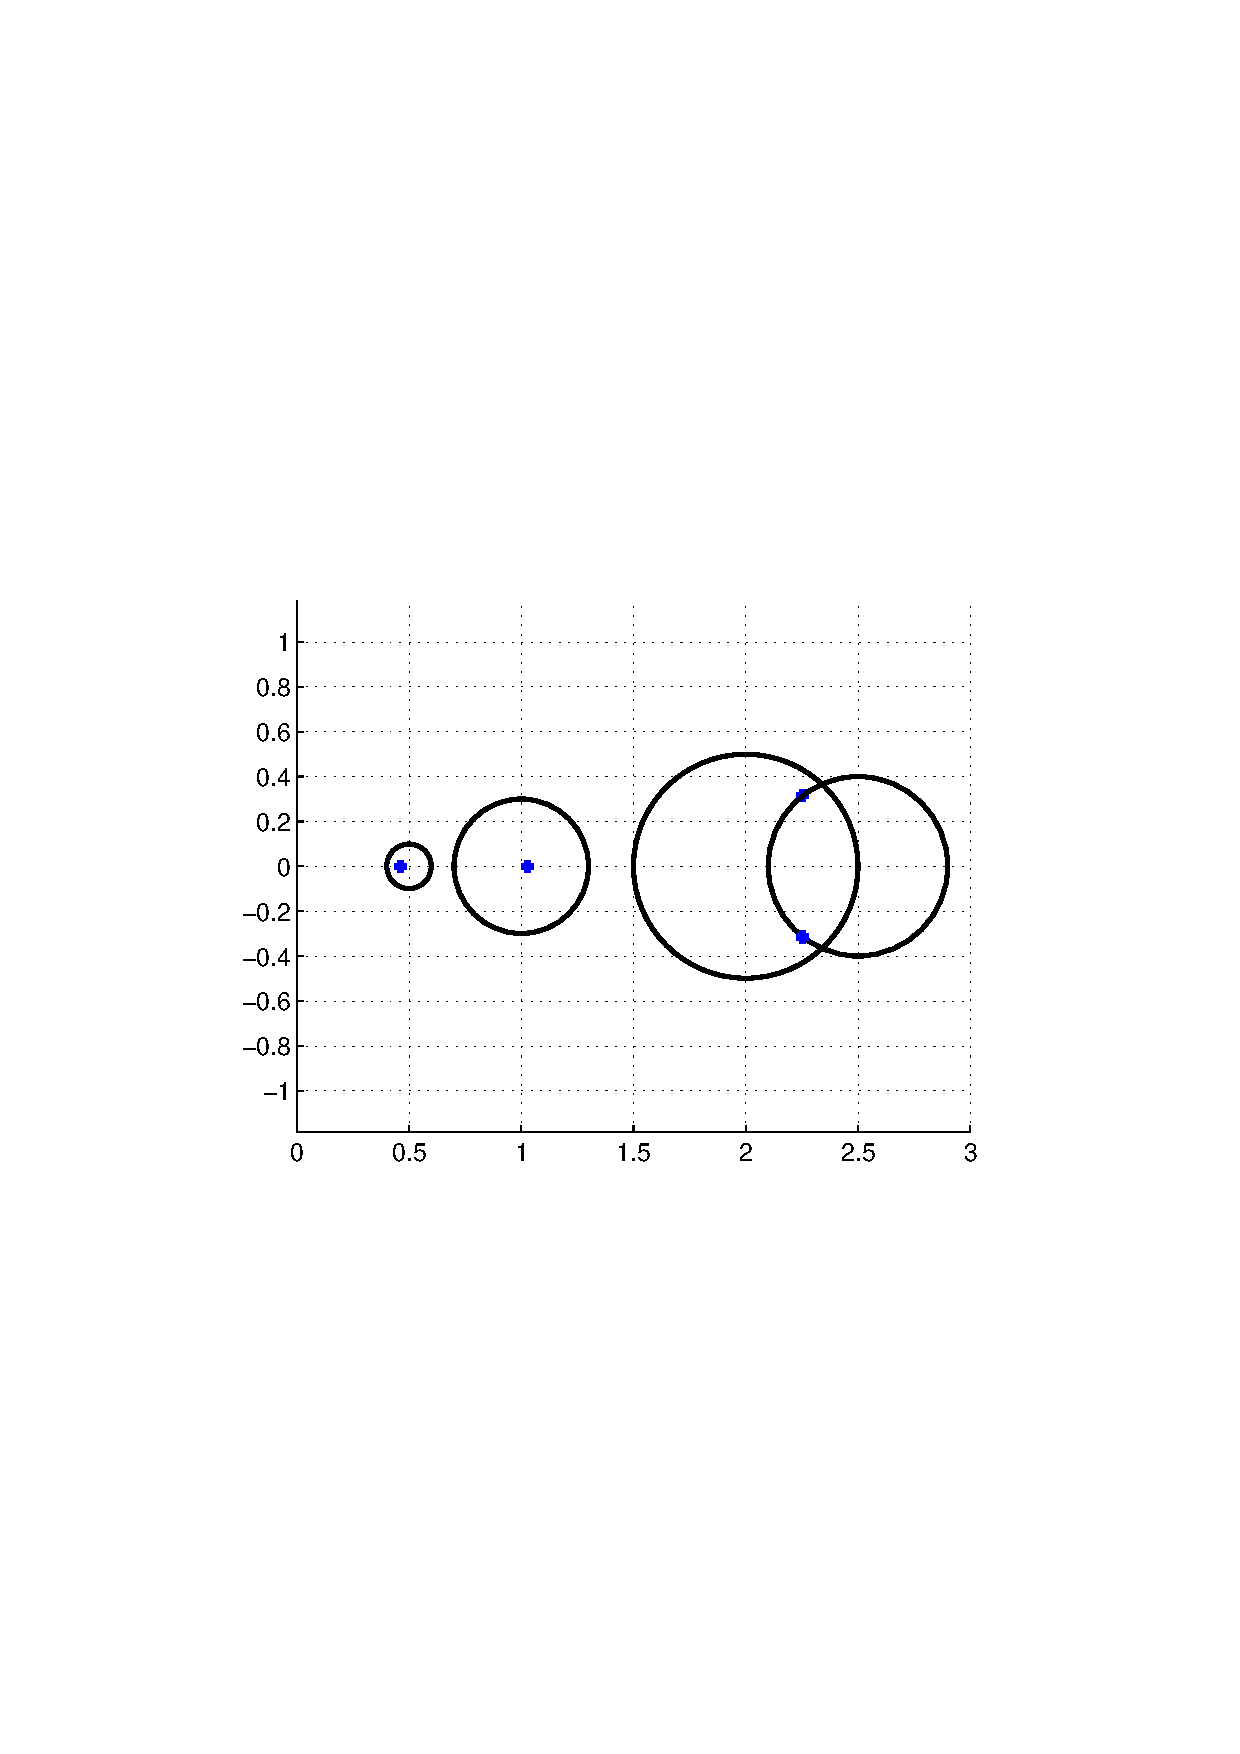
\includegraphics[width = \columnwidth]{gersh.pdf}
\end{minipage}

{\color{red}\bf Exercice 9.}
Si l'union de~$k$ disques de Gershgorin est disjointe avec l'union des
autres~$n-k$ disques, alors la première union contient exactement~$k$ valeurs
propres et la deuxième~$n-k$.

{\bf Corollaire.}
Si les disques de Gerschgorin sont deux-à-deux disjoints alors la matrice est
diagonalisable.

%{\bf Proposition.}
%Soit~$A$ une matrice irréductible et fortement diagonale dominante
%($\ \abs{a_{ii}}\ge\sum_{i\neq j}\abs{a_{ij}}$ avec au moins une inégalité
%stricte).  Alors~$A$ est inversible.  Si~$A$ est réductible en~$k$ blocs,
%une condition suffisante d'inversibilité est qu'il y ait~$k$ inégalités
%strictes, une dans chaque bloc.

\end{frame}

% décomposition polaire
\begin{frame}
DÉCOMPOSITION POLAIRE\\
=====================

{\bf Proposition.}
Toute matrice inversible~$A\in\GL_n(\C)$ admet une {\color{blue}décomposition
polaire} unique et continue~$A=HQ$ avec~$H\in\HH_n^{++}(\C)$
et~$Q\in\UU_n(\C)$.
%L'application~$A\mapsto(H,Q)$ est un homéomorphisme entre~$\GL_n(\C)$
%et~$\HH_n^{++}(\C)\times\UU_n(\C)$.\\
%Si~$A$ est réelle, alors~$H$ et~$Q$ le sont
%aussi (et donc~$H\in\SSS^{++}_n(\R)$ et~$Q\in\OO_n(\R)$).

{\bf Analogie.}~$H$ est le ``rayon'', une matrice positive.\\
$Q$ est l'``angle'', une matrice unitaire.

{\color{red}\bf Exercice 12.} Démontrez la proposition.

{\color{red}\bf Exercice 13.}
Calculez la décomposition polaire de la
matrice~$A=\parens{\begin{smallmatrix}1&1\\0&1\end{smallmatrix}}$.
\end{frame}

% décomposition en valeurs singulières
\begin{frame}
DÉCOMPOSITION EN VALEURS SINGULIÈRES (SVD)\\
==========================================

\emph{\small\sl Every matrix is diagonal, provided one uses the proper bases for
the domain and range spaces.\\ \hfill---Gilbert Strang}

\pause
{\bf Proposition (décomposition SVD).}
	Soit~$A\in\M_{p,q}(\C)$.  Alors il existent deux matrices unitaires~$U\in
	\UU_p(\C)$, $V\in\UU_q(\C)$ et une matrice quasi-diagonale~$\Sigma\in
	\M_{p,q}(\C)$
	\[
		\Sigma = \parens{\begin{smallmatrix}
			\sigma_1 & & & & \\
			 & \ddots & & & \\
			 & & \sigma_r & & \\
			 & & & 0 & \\
			 & & & & \ddots
	 \end{smallmatrix}}
	\]
	telles que~\fbox{$A=U\/\Sigma V^*$}.  Les nombres réels
	positifs~$\sigma_i$ sont les valeurs singulières non nulles de~$A$.\\
	En particulier,~$r$ est le rang de~$A$. \\
%	Si~$A$ est réelle alors on peut choisir~$U$ et~$V$ réelles orthogonales.
\end{frame}

% pseudo-inverse de Moore-Penrose
\begin{frame}
PSEUDO-INVERSE DE MOORE-PENROSE\\
===============================

{\bf Objectif:} résoudre de façon canonique le système~$Ax=b$,
quel que soit la taille et le rang de~$A\in\M_{m,n}(\K)$.

{\bf Définition.}
Soit~$A\in\M_{p,q}(\C)$ et~$A=U\/\Sigma V^*$ sa SVD
avec~$U\in\UU(p)$, ~$V\in\UU(q)$
et~$\Sigma=\parens{\begin{smallmatrix}D&0\\0&0\end{smallmatrix}}$.
La~\emph{pseudo-inverse} de~$A$ est la matrice~$A\in\M_{q,p}(\C)$ définie
par
\[
	A^+=V\Sigma^+ U^*
	\qquad
	\textrm{avec}
	\qquad
	\Sigma^+=\begin{pmatrix}D^{-1}&0\\0&0\end{pmatrix}
\]
\pause
{\bf\color{red} Exercice 14.} La pseudo-inverse ``généralise l'inverse''\\
{\bf\color{red} Exercice 15.} Elle généralise aussi les moindres carrés\\
{\bf\color{red} Exercice 15.} Calculez les pseudo-inverses de:\\\vspace{-.5em}
	\begin{itemize}
		\item Un scalaire~$a\in\K=\M_{1,1}(\K)$.
		\item Un vecteur ligne ou colonne~$\x\in\K^n\approx\M_{n,1}(\K)\approx\M_{1,n}(\K)$ 
		\item Les matrices~$\parens{\begin{smallmatrix}0&1\\0&0\end{smallmatrix}}$,
			$\parens{\begin{smallmatrix}1&1\\1&1\end{smallmatrix}}$ et~$\x\x^*\in\M_{n,n}(\K)$ avec~$\x\in\K^n$.
	\end{itemize}



\end{frame}


%% normes matricielles, définition, propriétés, exemples
%\begin{frame}
%ENSEMBLES DE MATRICES\\
%=====================
%\end{frame}
%
%% normes et rayon spectral
%\begin{frame}
%ENSEMBLES DE MATRICES\\
%=====================
%\end{frame}
%
%% théorème de Houseolder
%\begin{frame}
%ENSEMBLES DE MATRICES\\
%=====================
%\end{frame}
%
%% convergence de suites de matrices
%\begin{frame}
%ENSEMBLES DE MATRICES\\
%=====================
%\end{frame}
%
%% conditionement, erreurs d'observation et de modélisation
%\begin{frame}
%ENSEMBLES DE MATRICES\\
%=====================
%\end{frame}


\begin{frame}
REPARTITION DES EXERCICES\\
=========================

{\bf Tous:} Exercices 1, 2 (intersection de groupes) et 5.\\
{\bf Groupe 1:} Exercice 3 (théorème spectral)\\
{\bf Groupe 2:} Exercices 4 et 6 (éléments propres)\\
{\bf Groupe 3:} Exercice 7 (théorème du min-max)\\
{\bf Groupe 4:} Exercice 8 et 9 (disques de Gershgorin)\\
{\bf Groupe 5:} Exercice 12 et 13 (décomposition polaire)\\
{\bf Groupe 6:} Exercice 14, 15 et 17 (pseudo-inverse)\\


\vfill
Temps:\\
{\bf 90min} travail en groupe (6 groupes de 2,3,4 personnes)\\
{\bf 60min} mise en commun
(6 présentations de 10min par les ``scribes'' de chaque groupe)

\end{frame}

\end{document}


% vim:sw=2 ts=2 spell spelllang=fr:
